% !TeX program = xelatex
% Build: latexmk -xelatex -interaction=nonstopmode -halt-on-error -file-line-error -cd Report/report.tex
% Body layout: the supplied Basic Academic Journal Article Template (olplainarticle).
% Cover layout: the authors' supplied University of St. Gallen example.
% Word sources are transcribed into parts/; neither Word files nor the ZIP are
% required to compile. The bibliography is followed by the list of aids and
% the declaration of authorship.
\documentclass[11pt]{olplainarticle}
% Author-requested symmetric 2 cm side margins on A4.
\geometry{a4paper,left=2cm,right=2cm,headheight=14pt}
\usepackage{fontspec}
\setmainfont{texgyretermes}[
  Extension=.otf,UprightFont=*-regular,ItalicFont=*-italic,
  BoldFont=*-bold,BoldItalicFont=*-bolditalic,Ligatures=NoCommon,Mapping=]
\setsansfont{texgyreheros}[
  Extension=.otf,UprightFont=*-regular,ItalicFont=*-italic,
  BoldFont=*-bold,BoldItalicFont=*-bolditalic,Ligatures=NoCommon,Mapping=]
\setmonofont{lmmono10-regular.otf}[Scale=MatchLowercase]
\usepackage{setspace}
\onehalfspacing
\usepackage{tabularx,array}
\usepackage{xurl}
\usepackage{hyperref}
\definecolor{HSGGreen}{HTML}{00843D}
\hypersetup{
  pdftitle={Can Approval-Day Information Predict Interruptions of Conditional Lending Programmes?},
  pdfauthor={Mathis Clément; Ethan Moore; Ali Haidar; Tristan Zemp; Joao Matteo Pisaturo; José Pablo Caldas; Federico Marcelli},
  pdfsubject={Approval-day prediction of conditional lending programme interruptions},
  colorlinks=true,linkcolor=color1,citecolor=color1,urlcolor=HSGGreen
}
% Show only the current page number in the footer.
\rfoot{\small\sffamily\bfseries\thepage}
\setlength{\tabcolsep}{4pt}
\renewcommand{\arraystretch}{1.24}
\setlength{\parskip}{4pt plus 1pt minus 1pt}
\setlength{\emergencystretch}{2em}
\setlength{\skip\footins}{12pt plus 2pt minus 1pt}
\titlespacing*{\section}{0pt}{20pt plus 3pt minus 2pt}{9pt plus 2pt minus 1pt}
\titlespacing*{\subsection}{0pt}{14pt plus 2pt minus 1pt}{6pt plus 1pt}
\titlespacing*{\subsubsection}{0pt}{12pt plus 2pt minus 1pt}{5pt plus 1pt}
\widowpenalty=10000
\clubpenalty=10000
\raggedbottom
\newcolumntype{L}[1]{>{\raggedright\arraybackslash}p{#1}}

% Identity wrappers retain source text for fidelity checks.
\newcommand{\src}[1]{#1}
\newcommand{\srcnote}[1]{#1}
\newcommand{\addsec}[1]{\section*{#1}\phantomsection\addcontentsline{toc}{section}{#1}}
\newcommand{\addsubsec}[1]{\subsection*{#1}\phantomsection\addcontentsline{toc}{subsection}{#1}}
\newcommand{\wordcaption}[1]{\par\addvspace{6pt}{\noindent\sffamily\small\color{color1}#1\par}\addvspace{6pt}}
\newcommand{\wordtablecaption}[2]{%
  \refstepcounter{table}\label{#1}%
  \wordcaption{#2}}
\newenvironment{wordtable}{%
  \par\addvspace{10pt}\setlength{\parfillskip}{0pt plus 1fil}%
  \noindent\begin{minipage}{\linewidth}\singlespacing\small
  \setlength{\parskip}{0pt}\setlength{\parindent}{0pt}%
}{\end{minipage}\par\addvspace{10pt}}
\newenvironment{wordreferences}{%
  \begingroup\singlespacing\small\setlength{\parskip}{5pt}%
  \setlength{\parindent}{0pt}\everypar{\hangindent=1em\hangafter=1}%
}{\par\endgroup}

\title{Can Approval-Day Information Predict Interruptions of Conditional Lending Programmes?}
\newcommand{\reportauthors}{%
  Mathis Clément\par
  Ethan Moore\par
  Ali Haidar\par
  Tristan Zemp\par
  Joao Matteo Pisaturo\par
  José Pablo Caldas\par
  Federico Marcelli\par}
\author{\reportauthors}
\affil{University of St. Gallen}
\date{Wednesday, 14 October 2026}
\newcommand{\reportcourse}{5,155,1.00 Machine Learning in Finance}
\newcommand{\reportinstructor}{Prof. Dr. Despoina Makariou}
\newcommand{\reportgroup}{6}

% Standalone cover following the supplied example.
\makeatletter
\renewcommand{\maketitle}{%
  \begingroup
  \thispagestyle{empty}
  \singlespacing\normalfont
  \setlength{\parindent}{0pt}\setlength{\parskip}{0pt}
  \vspace*{-5mm}
  {\centering
    % Crop the symbol from the existing 788 x 170 px, 96 dpi HSG wordmark.
    
\includegraphics[height=19mm,viewport=0 0 116 128,clip]{../Presentation/figures/hsg_logo.png}\par
    \vspace{4mm}
    {\bfseries\fontsize{24}{28}\selectfont University of St. Gallen\par}
    \vspace{4mm}
    {\fontsize{11}{18}\selectfont
      University of Business, Economics, Law, Social Sciences, International Affairs and\\
      Computer Science (HSG)\par}
  }
  \vspace{10mm}
  \hrule height 0.4pt
  \vspace{4mm}
  {\centering
    {\fontsize{18}{27}\selectfont\@title\par}
    \vspace{4mm}
    {\fontsize{11}{15}\selectfont
      A Comparison of Random Forests, Logistic Regression and Neural Networks\par}
  }
  \vspace{5mm}
  \hrule height 0.4pt
  \vspace{28mm}
  {\fontsize{12}{18}\selectfont
    \renewcommand{\arraystretch}{1}
    \begin{tabularx}{\linewidth}{@{}>{\bfseries}L{48mm}@{\hspace{5mm}}>{\raggedright\arraybackslash}X@{}}
      Course: & \reportcourse\\[10mm]
      Instructor: & \reportinstructor\\[10mm]
      Submission date: & \@date\\[10mm]
      Group \reportgroup: & {\fontsize{12}{20}\selectfont\reportauthors}\\
    \end{tabularx}\par
  }
  \endgroup
}
\makeatother

\begin{document}
\maketitle
\thispagestyle{empty}
\clearpage
\tableofcontents
\clearpage
% Revised under the editorial brief; template formatting is unchanged.
\section{\src{Introduction and related literature}}\label{sec:introduction}
\subsection{\src{Motivation and financial relevance}}\label{sec:motivation}

\src{Many official lenders provide conditional financing: they disburse a loan in tranches and release each tranche after the first only when a review confirms that the borrower is meeting the policy conditions agreed at approval. The World Bank’s development policy financing and the European Union’s macro-financial assistance, for example, also attach policy conditions to their loans. We study interruption risk using programmes of the International Monetary Fund (IMF), which form a natural sample: the IMF’s Monitoring of Fund Arrangements database (MONA) records the review schedule of IMF-supported programmes approved since 2002 and whether each review was completed (IMF, 2026b), which gives a consistent record at the programme level.}

\src{The IMF supports countries facing balance-of-payments difficulties through lending programmes that combine financing with policy commitments and periodic reviews. We ask whether information available at approval by the IMF Executive Board (the Board) can predict whether a programme is later interrupted (see Section~\ref{sec:prediction-task} for the outcome definition).}

\src{Interruption matters financially because implementation can affect expected financing and confidence in the government’s policy commitments. Mody and Saravia (2006, pp. 843–845, 857) find that IMF programmes do not uniformly improve access to international bond markets; favourable effects depend on credible reform commitments and economic circumstances. Reinsberg et al. (2022, pp. 1023, 1034–1035) associate permanent interruptions with lower institutional investor ratings and a short-lived increase in sovereign bond spreads.}

\subsection{\src{Political incentives and implementation capacity}}\label{sec:political-incentives}

\src{The implementation literature emphasises the borrowing government’s willingness and ability to fulfil its commitments. Ivanova et al. (2003, pp. 4, 34) identify political cohesion, stability and bureaucratic quality as important influences on implementation. Joyce (2006, pp. 342–345, 351) similarly links implementation to government ideological cohesion, regime duration and political and economic openness. Dreher (2003, pp. 101, 111–114) shows that electoral incentives interact with political institutions and also identifies associations with initial economic vulnerability.}

\src{Our 13 inputs do not directly measure elections, political cohesion or bureaucratic quality, so these mechanisms are only partly observed.}

\subsection{\src{Conditionality and programme design}}\label{sec:conditionality}

\src{Evidence on conditionality is mixed. Ivanova et al. (2003, pp. 4, 34) find limited explanatory power for conditionality once domestic political factors are considered. Dreher’s (2009, pp. 248–250) survey discusses competing arguments about conditions as commitment devices and constraints on implementation. More recently, Reinsberg et al. (2022, pp. 1023, 1026, 1035) find that greater structural conditionality at programme onset is associated with interruption, especially conditions involving public-sector reform, privatisation and price liberalisation.}

\src{The outcome definition also affects interpretation, because duration and review counts may predict interruption partly through exposure (Section~\ref{sec:variables}). Counting conditions also misses their political difficulty and content.}

\subsection{\src{Macroeconomic vulnerability and prior programme use}}\label{sec:prior-use}

\src{Weak growth, inflation and external financing pressures can make agreed adjustment harder to implement. Iseringhausen et al. (2019, pp. 8, 16, 19, 23–25) find that macroeconomic conditions, institutions and previous IMF experience help explain repeated programme use. Their outcome, however, is a successor arrangement within three years. A country can return to the IMF after successfully completing a programme because it experiences a new shock.}

\subsection{\src{Machine learning in related work and our contribution}}\label{sec:contribution}

\src{Machine learning already contributes to IMF forecasting. Agbloyor et al. (2023, pp. 1–5) predict IMF bailouts using 6,550 observations and 138 features, reporting predictive information from economic, agricultural, energy, health and social indicators. Batsuuri et al. (2024, pp. 12, 14–18, 22–25) find that machine-learning methods outperform traditional approaches when forecasting new IMF arrangements, with results sensitive to preprocessing and prediction horizon. Both studies predict participation; we predict what happens after a programme is approved.}

\src{Gu et al. (2020, pp. 2223, 2225–2227) demonstrate the value of non-linearities and interactions in equity-return prediction. Their large stock-return panel differs from our 173-programme sample, so gains from flexibility may not carry over; logistic regression provides a benchmark. Breiman (2001a, pp. 5–8, 10–11) provides the basis for random forests, which combine predictions from randomised trees. We compare the random forest with logistic regression, an interpretable benchmark for a binary outcome, and a neural network.}

\src{Our contribution is a focused predictive test, in the sense of Shmueli (2010), of the research question stated in Section~\ref{sec:prediction-task}. The literature covers implementation mechanisms, financial consequences, predictors of participation or repeated use, and the determinants of interruption, but to our knowledge no study evaluates out-of-sample prediction of interruption with approval-day information.}

% The reviewed study-design wording is retained where the brief's OLD text is absent.
\section{\src{Research design}}\label{sec:design}
\subsection{\src{Research question and prediction task}}\label{sec:prediction-task}

\src{The general question of this study is whether the information available on the day a conditional lending programme is approved can predict whether the programme will later be interrupted, and whether a flexible model such as a random forest predicts this better than logistic regression or a neural network. We use IMF programmes as the sample for this analysis, because MONA records the scheduled and completed reviews of IMF-supported programmes approved since 2002 (Section~\ref{sec:motivation}). We test whether approval-day information can predict if an IMF programme will be interrupted. The unit of observation is one lending programme. The prediction is made at Board approval, using only data known on that date.}

\src{This is a supervised binary classification task. The output equals 1 when fewer reviews were completed than scheduled at approval. It equals 0 when every scheduled review was completed. The inputs are 13 variables in four groups: deal structure, conditionality, track record and macroeconomic conditions. Section~\ref{sec:variables} lists them.}

\src{Following James et al. (2013, pp. 16–17), we estimate f in Pr(Y = 1 | X) = f(X). The estimate is judged on programmes it has not seen during training. Following Shmueli (2010, p. 291), we treat this as a prediction problem. Coefficients and variable importance are not read as causal effects.}

\src{Performance is measured on a later test set, with interrupted programmes as the positive class. We report accuracy; sensitivity, the share of interrupted programmes the model flags; specificity, the share of completed programmes it correctly clears; and balanced accuracy, the mean of sensitivity and specificity (Brodersen et al., 2010, p. 3121). We also report the area under the receiver operating characteristic curve (AUC), the probability that a model ranks a randomly chosen interrupted programme above a randomly chosen completed one, so 0.500 corresponds to random guessing (Fawcett, 2006, p. 867). Interruptions are the majority in the test set (see Section~\ref{sec:sample}). A rule that always predicts interruption therefore gets high accuracy. Its balanced accuracy is only 0.500. Plain accuracy misleads when classes are unequal (He \& Garcia, 2009, p. 1276). Balanced accuracy removes this advantage. The random forest and the neural network are tuned on balanced accuracy for the same reason; the logistic regression is not tuned.}

\src{The IMF pays its financing in tranches. Each tranche after the first requires the Board to complete a scheduled review (IMF, n.d.). The review checks the quantitative targets and structural conditions agreed at approval. When a review is not completed, the next disbursement is withheld. The country then loses financing the programme had scheduled. An approval-day flag would, if accurate, inform programme design at the IMF and risk assessment by creditors; Section~\ref{sec:policy} discusses whether our results support such a flag.}

\subsection{\src{Study design, data sources and train/test split}}\label{sec:data-sources}

\src{The study is a cross-section of IMF programmes. Each row is one programme, described as it stood at approval. We keep facilities with scheduled reviews, including their predecessors. These are the Stand-By Arrangement (SBA), the Extended Fund Facility (EFF), the Extended Credit Facility (ECF), and the Standby Credit Facility (SCF). The ECF and the SCF are concessional facilities of the IMF’s Poverty Reduction and Growth Trust (PRGT). Facilities without reviews and precautionary arrangements are dropped (see Section~\ref{sec:sample}). Approvals run from 2002 to 2016. Review records in MONA start in 2002. Ending the window in 2016 limits overlap with the COVID-19 period.}

\src{No single public source records programme design and review outcomes together. We therefore built the dataset from IMF files. The IMF Financial Data Query Tool gives the history of lending arrangements (IMF, 2026a); we call this source the commitments file. It provides dates, facility type, and access in percent of quota at approval. MONA covers reviews, conditions, and staff macro estimates (IMF, 2026b). We use four MONA files. Reviews lists scheduled and completed reviews, from which we build the output. Combined lists structural conditions and prior actions. Mecon holds staff estimates of growth, inflation, and the current account. Description holds a cancellation flag, used only to check the output. We also downloaded the April 2026 World Economic Outlook (WEO; IMF, 2026c). We also used the World Bank’s World Development Indicators (WDI; World Bank, 2026). The final macro inputs come from MONA; Section~\ref{sec:variables} explains why.}

\src{The commitments file and MONA share no common identifier. Country names are spelled differently, and approval dates can differ by a few days. We normalise country names and match on the closest approval date within 60 days. Blends, in which two facilities (for example an ECF and an EFF) are approved for the same country on the same day, become one programme, because they share one review schedule. Overlapping or successive programmes of the same country are kept as separate observations (Section~\ref{sec:limitations}). Section~\ref{sec:sample} reports the resulting sample.}

\src{We split the sample by approval year. Training covers 2002 to 2013, and the test set covers 2014 to 2016. The test programmes are never used to fit or tune the models. All inputs are taken as they stood on approval day (see Section~\ref{sec:variables}). Hyperparameters are tuned on the training set with 10-fold cross-validation (CV) and leave-one-out cross-validation (LOOCV). A third scheme, country-grouped 10-fold CV (country CV), holds out whole countries in each fold. Many countries have several programmes, so random folds put one country on both sides. Randomly split folds give over-optimistic error estimates and favour overly complex models when observations are dependent (Roberts et al., 2017, p. 914). We use the country-grouped scores to choose the tuned settings for the random forest and the neural network. A prediction for a programme from a model fitted without that programme is called an out-of-fold prediction.}

% Data-section revisions specified in the editorial brief.
\section{\src{Data}}\label{sec:data}
\subsection{\src{Sample construction and summary statistics}}\label{sec:sample}

\src{Our final dataset covers 173 IMF lending programmes in 86 countries, approved between 2002 and 2016; 82 of them (47.4\%) were interrupted.}

\src{Starting from the 1,576 lending arrangements since 1952 in the commitments file, we keep the 221 non-precautionary arrangements approved in 2002–2016. We drop rapid one-off loans under the Rapid Credit Facility (RCF) and the Rapid Financing Instrument (RFI), which have no review schedule and so cannot be interrupted, and the Precautionary and Liquidity Line (PLL), a precautionary instrument. Merging blended programmes into one observation leaves 182 programmes, of which 173 match MONA. We split by approval year (training 2002–2013, \emph{n} = 145; test 2014–2016, \emph{n} = 28) and fill the few missing values with training-set medians, so nothing from the test period leaks into training. Table~\ref{tab:summary} summarises the 13 inputs.}

% Keep the two data tables together in one floating block.
\begin{table}[htbp]
\begin{wordtable}
\wordtablecaption{tab:summary}{\src{Table \thetable. Summary statistics of the 13 inputs (before imputation, \emph{n} = 173)}}
\begin{tabularx}{\linewidth}{@{}lXrrrrrr@{}}
\toprule
\src{Variable} & \src{Unit} & \src{Missing} & \src{Mean} & \src{SD} & \src{Min} & \src{Median} & \src{Max}\\
\midrule
\src{log\_access\_pct\_quota} & \src{log of \% of quota} & \src{0} & \src{4.62} & \src{1.29} & \src{1.61} & \src{4.50} & \src{8.08}\\
\src{planned\_months} & \src{months} & \src{0} & \src{32.58} & \src{7.56} & \src{7.20} & \src{35.98} & \src{47.97}\\
\src{n\_reviews\_sched} & \src{count} & \src{0} & \src{6.60} & \src{2.27} & \src{2.00} & \src{6.00} & \src{16.00}\\
\src{n\_struct\_cond} & \src{count} & \src{1} & \src{10.67} & \src{4.98} & \src{2.00} & \src{10.00} & \src{26.00}\\
\src{n\_prior\_actions} & \src{count} & \src{1} & \src{2.79} & \src{2.98} & \src{0.00} & \src{2.00} & \src{16.00}\\
\src{prev\_n\_20y} & \src{count} & \src{0} & \src{3.35} & \src{2.06} & \src{0.00} & \src{3.00} & \src{8.00}\\
\src{years\_since\_prev} & \src{years} & \src{11} & \src{4.09} & \src{6.82} & \src{0.00} & \src{1.62} & \src{47.74}\\
\src{growth} & \src{\%} & \src{5} & \src{4.04} & \src{4.23} & \src{−8.69} & \src{4.15} & \src{24.46}\\
\src{inflation} & \src{\%} & \src{8} & \src{7.73} & \src{7.93} & \src{−17.69} & \src{5.50} & \src{48.04}\\
\src{current\_account\_gdp} & \src{\% of GDP} & \src{10} & \src{−8.62} & \src{11.77} & \src{−92.49} & \src{−6.20} & \src{15.36}\\
\src{concessional} & \src{0/1} & \src{0} & \src{0.64} & \src{0.48} & \src{0.00} & \src{1.00} & \src{1.00}\\
\src{extended} & \src{0/1} & \src{0} & \src{0.69} & \src{0.46} & \src{0.00} & \src{1.00} & \src{1.00}\\
\src{no\_track\_record} & \src{0/1} & \src{0} & \src{0.06} & \src{0.25} & \src{0.00} & \src{0.00} & \src{1.00}\\
\bottomrule
\end{tabularx}
\par\smallskip
{\footnotesize\itshape\src{Note. For binary variables the mean is the share of programmes with value 1. Variable names are explained in Table~\ref{tab:variables}. Source: authors’ calculations from IMF MONA and lending-arrangements data.}\par}
\end{wordtable}

\begin{wordtable}
\footnotesize
\renewcommand{\arraystretch}{1.05}
\wordtablecaption{tab:variables}{\src{Table \thetable. Input and output variables}}
\begin{tabularx}{\linewidth}{@{}L{0.23\linewidth}L{0.17\linewidth}>{\raggedright\arraybackslash}XL{0.23\linewidth}@{}}
\toprule
\src{Variable} & \src{Group} & \src{Description} & \src{Source}\\
\midrule
\src{interrupted} & \src{Output} & \src{1 = fewer reviews completed than scheduled at approval} & \src{MONA Reviews}\\
\src{log\_access\_pct\_quota} & \src{Deal structure} & \src{Log of agreed access, \% of IMF quota} & \src{Commitments file, upon approval}\\
\src{planned\_months} & \src{Deal structure} & \src{Planned length, approval to scheduled expiry} & \src{Commitments file, upon approval}\\
\src{concessional} & \src{Deal structure} & \src{1 = includes a concessional (PRGT) facility} & \src{Commitments file}\\
\src{extended} & \src{Deal structure} & \src{1 = EFF or ECF} & \src{Commitments file}\\
\src{n\_reviews\_sched} & \src{Deal structure} & \src{Reviews scheduled at approval} & \src{MONA Reviews, R0}\\
\src{n\_struct\_cond} & \src{Conditionality} & \src{Structural conditions at approval} & \src{MONA Combined, R0}\\
\src{n\_prior\_actions} & \src{Conditionality} & \src{Prior actions before Board approval} & \src{MONA Combined, R0}\\
\src{prev\_n\_20y} & \src{Track record} & \src{Programmes in the 20 years before approval} & \src{Commitments file, history}\\
\src{years\_since\_prev} & \src{Track record} & \src{Years since the previous programme’s planned end (0 if overlapping)} & \src{Commitments file, history}\\
\src{no\_track\_record} & \src{Track record} & \src{1 = no earlier programme} & \src{Commitments file, history}\\
\src{growth} & \src{Macro\-economic} & \src{Real GDP growth, \%, staff estimate for the approval year} & \src{MONA Mecon, R0}\\
\src{inflation} & \src{Macro\-economic} & \src{CPI inflation, \%, staff estimate for the approval year} & \src{MONA Mecon, R0}\\
\src{current\_account\_gdp} & \src{Macro\-economic} & \src{Current-account balance, \% of GDP} & \src{MONA Mecon, R0}\\
\bottomrule
\end{tabularx}
\par\smallskip
{\footnotesize\src{Note. R0 = MONA’s approval snapshot. PRGT = Poverty Reduction and Growth Trust. EFF = Extended Fund Facility; ECF = Extended Credit Facility.}\par}
\end{wordtable}
\end{table}

\src{The classes are close to balanced overall, but interruptions rise from 39\% of approvals in 2002–2004 to 61\% in 2014–2016. They are the minority in training (65 of 145, 44.8\%) and the majority in the test set (17 of 28, 60.7\%). Always predicting “interrupted” would therefore already be right for 60.7\% of test programmes, which is the accuracy benchmark; on balanced accuracy, the metric we use, this rule scores 0.500.}

\src{ECFs, concessional loans to low-income countries, make up 97 of the 173 programmes, followed by 47 SBAs, 16 EFFs, 8 blends and 5 SCFs. Interruption rates range from 64\% for SBAs to 38\% for ECFs and blends.}

\src{A typical programme runs for three years with six scheduled reviews, ten structural conditions and two prior actions. Access in percent of quota is strongly right-skewed, so we use its log, and the macro variables have long tails (inflation runs from −18\% to 48\%). A few extreme macro values (e.g. Yemen’s 2014 inflation of −17.7\%) may reflect recording issues in MONA. Missing values are rare: the time since the previous programme is undefined for the 11 first-time borrowers, and no other input misses more than 10 values. Each missing value is filled with the median of the 145 training programmes, and the test set uses the same training medians. For the 11 first-time borrowers, the time since the previous programme is set to the training median of 1.6 years; the no-track-record indicator equals 1 for exactly these programmes, so the models can distinguish them from countries that returned after a short gap. The medians are computed once on the full training set, so the cross-validation folds share them; with at most 11 missing values per input, this effect on the cross-validation scores is small.}

\src{Across all 173 programmes, interrupted programmes differ from completed ones mainly in deal structure, although planned length differs little. They schedule more reviews (7.3 against 5.9), receive more access relative to quota (mean log access 4.96 against 4.31) and are less often concessional (52\% against 74\%) or extended (59\% against 79\%), all with Welch \emph{t}-test \emph{p}-values below 0.01. Gaps in conditionality, track record and macroeconomic conditions are smaller, with Welch \emph{t}-test \emph{p}-values of 0.09 or more.}

\subsection{\src{Output and input variables}}\label{sec:variables}

\src{The output is whether a programme was interrupted. All 13 inputs are known on the day the Board approves the programme, which is when the prediction is made.}

\src{\textbf{Selection principle.} A predictive input must be available at the time of prediction and carry information about the outcome; it needs no causal interpretation (Shmueli, 2010). We therefore use only approval-day information: the “upon approval” columns of the commitments file and MONA’s approval snapshot (R0).}

\src{\textbf{Output.} Tying the label to the approval-day review schedule means later rescheduling cannot change it. MONA’s cancellation flag would be too narrow: only 29 of the 82 interrupted programmes were formally cancelled, while the other 53 ended with reviews outstanding.}

\src{\textbf{Inputs.} Table~\ref{tab:variables} groups the inputs into deal structure, conditionality, track record and macroeconomic conditions.}

\src{\textbf{Transformations and overlap.} Access enters in logs. Facility type is left out because the concessional and extended indicators identify it exactly, and the number of tranches because it is almost always the number of reviews plus one. Some inputs remain correlated (the extended indicator with planned length, \emph{r} = 0.77; the extended indicator with the concessional indicator, \emph{r} = 0.81), which matters little for the forest’s predictions but makes the importance of each input and the logistic regression coefficients harder to read.}

\src{\textbf{Excluded variables.} Post-approval outcomes and identifiers are excluded, as are fiscal variables: the April 2026 World Economic Outlook contains revised rather than approval-day values (IMF, 2026c), and MONA lacks them for 24–45\% of programmes. The full exclusions are listed in the supplementary Excel file submitted with this report.}

\src{\textbf{Caveats.} The number of scheduled reviews enters both an input and the outcome definition, so part of its predictive power is mechanical. The macro inputs are staff projections at approval, which may be optimistic but are what was known at the time.}

% Minimal sentence-level revisions: C-61 to C-97 and the specified global edits.
\section{\src{Random forest}}\label{sec:forest}
\subsection{\src{Method, tuning and test predictions}}\label{sec:forest-method}

\src{\textbf{Method.} The first model is a random forest. Because our study is a classification problem, a random forest appeared a promising starting point (Batsuuri et al., 2024, p. 3). This model combines many classification trees, each splitting the data through a series of simple yes/no questions.}

\src{A single tree captures non-linear patterns and interactions, but it is unstable: small changes in the data can produce a very different tree. For this reason, we use bagging (bootstrap aggregation). The idea is to grow many trees, each on a bootstrap sample (programmes drawn with replacement), and average their votes. Averaging helps to cancel out noisy predictions. However, bagging alone has a weakness. If one input is very strong, almost every tree will split on it first, making the trees similar, which limits the gain from averaging (James et al., 2013, p. 320). Indeed, Hastie et al. (2009, p. 588) formalised it with the variance of an average of B trees, each with variance σ² and pairwise correlation ρ:}

\begin{equation}
\label{eq:forest-variance}
\operatorname{Var}=\rho\sigma^2+\frac{(1-\rho)\sigma^2}{B}
\end{equation}

\src{More trees (B) shrink the second term, but the first term only shrinks with less correlated trees. We use Breiman’s (2001a, p. 6) solution of limiting each split to a random subset of \emph{mtry} inputs. Each tree then votes: the share of trees voting “interrupted” gives the predicted probability, and a threshold assigns the class. The programmes left out of each bootstrap sample (out-of-bag, OOB) provide a built-in error estimate.}

\src{\textbf{Default forest.} The default forest was trained with the default hyperparameters of the \emph{randomForest} R package (Liaw \& Wiener, 2002): 500 trees, \emph{mtry} 3. Its OOB balanced accuracy is 0.609.}

\src{\textbf{Hyperparameter tuning.} To tune our hyperparameters (number of trees and \emph{mtry}), we scored 24 different pairs on balanced accuracy (Section~\ref{sec:prediction-task}), ranging from 100 to 1000 trees and \emph{mtry} from 2 to 12, with the \emph{caret} package (Kuhn, 2008).}

\src{We used three different cross-validation schemes: 10-fold CV, LOOCV and country-grouped 10-fold CV (country CV, Section~\ref{sec:data-sources}). The last is our main measurement, as it keeps all programmes of a country in the same fold, so the forest is never scored on a country it was trained on.}

\src{For 10-fold CV and country CV, we compute balanced accuracy within each fold and average over the ten folds; for LOOCV, where each fold holds a single programme, we compute it once over all out-of-fold predictions. Table~\ref{tab:rf-tuning} compares the default forest with the best pair under each scheme.}

\begin{wordtable}
\begin{tabularx}{\linewidth}{@{}>{\raggedright\arraybackslash}XL{0.22\linewidth}>{\raggedright\arraybackslash}XL{0.22\linewidth}@{}}
\toprule
\textbf{\src{Validation scheme}} & \textbf{\src{Default forest (500 trees, \emph{mtry} 3)}} & \textbf{\src{Best pair under this scheme}} & \textbf{\src{Balanced accuracy of best pair}}\\
\midrule
\src{Out-of-bag (default forest only)} & \src{0.609} & \src{n/a} & \src{n/a}\\
\src{10-fold CV} & \src{0.623} & \src{250 trees, \emph{mtry} 2} & \src{0.657}\\
\src{Country-grouped 10-fold CV} & \src{0.597} & \src{250 trees, \emph{mtry} 3} & \src{0.620}\\
\src{LOOCV} & \src{0.606} & \src{100 trees, \emph{mtry} 8} & \src{0.635}\\
\bottomrule
\end{tabularx}
\wordtablecaption{tab:rf-tuning}{\src{Table \thetable. Default against tuned forest on the training set (balanced accuracy; best of 24 pairs per scheme)}}
\end{wordtable}

\src{The default pair (500, 3) is part of the tuning grid, so its CV scores come from the same runs. OOB accuracy of the default forest is 0.628.}

\src{Country CV gives the lowest best score (0.620, against 0.657 for 10-fold CV and 0.635 for LOOCV), as expected, since the forest is never tested on a country it has seen. We still select it because it guards against within-country dependence (Section~\ref{sec:data-sources}), although 26 of the 28 test programmes come from countries seen in training, so it does not imitate the later-period test.}

\src{\textbf{Final model.} We keep the pair chosen under country CV (250 trees, \emph{mtry} 3), refit it on all 145 training programmes with the threshold that maximises out-of-fold balanced accuracy (0.51), and predict the 28 test programmes once (Table~\ref{tab:rf-results}). The selected pair keeps the default \emph{mtry} and only lowers the number of trees from 500 to 250, which cannot be expected to improve accuracy, so its gain over the default under country CV (0.620 against 0.597) most likely reflects noise in a search over 24 pairs. Only the test-set rows of Table~\ref{tab:rf-results} measure out-of-sample performance; the other figures in Tables~\ref{tab:rf-tuning} and~\ref{tab:rf-results} are training-set estimates used to choose settings.}

\begin{wordtable}
\begin{tabularx}{\linewidth}{@{}>{\raggedright\arraybackslash}XL{0.115\linewidth}L{0.12\linewidth}L{0.12\linewidth}L{0.13\linewidth}r@{}}
\toprule
\textbf{\src{Model}} & \textbf{\src{Accuracy}} & \textbf{\src{Sensitivity}} & \textbf{\src{Specificity}} & \textbf{\src{Balanced accuracy}} & \textbf{\src{AUC}}\\
\midrule
\src{Baseline (always interrupted)} & \src{0.607} & \src{1.000} & \src{0.000} & \src{0.500} & \src{0.500}\\
\addlinespace
\src{Default forest (threshold 0.50)} & \src{0.571} & \src{0.588} & \src{0.545} & \src{0.567} & \src{0.620}\\
\addlinespace
\src{Final forest (threshold 0.51)} & \src{0.500} & \src{0.471} & \src{0.545} & \src{0.508} & \src{0.586}\\
\addlinespace
\src{Final forest (threshold 0.50)}\footnotemark[1] & \src{0.571} & \src{0.588} & \src{0.545} & \src{0.567} & \src{0.586}\\
\midrule
\src{Final forest, training out-of-fold (\emph{n} = 145, threshold 0.51)} & \src{0.641} & \src{0.523} & \src{0.738} & \src{0.630} & \src{0.631}\\
\bottomrule
\end{tabularx}
\wordtablecaption{tab:rf-results}{\src{Table \thetable. Random forest on the test set (28 programmes, 2014–2016), with the final forest’s training out-of-fold scores for reference}}
\end{wordtable}
\footnotetext[1]{\srcnote{Note. Final forest: 250 trees, \emph{mtry} 3. The 0.50 row uses the same threshold as the logistic regression, for a like-for-like comparison; it differs from 0.51 only because two interrupted programmes sit at a vote share of 0.504. The last row is computed on the 145 training programmes, not on the test set.}}

\src{\textbf{Out-of-sample predictions.} On the 28 test programmes, the final forest reaches a balanced accuracy of 0.508, barely above the 0.500 of always predicting “interrupted”, and its accuracy (0.500) is even below that rule’s (0.607); the rule’s high accuracy despite zero skill shows why plain accuracy misleads when classes are unequal. Out of fold on the training set, it reaches 0.630; this is more precise than the test score but slightly optimistic, since both the pair and the threshold were chosen on these predictions. It differs from the 0.620 in Table~\ref{tab:rf-tuning} because that figure averages balanced accuracy over ten folds at threshold 0.50, whereas 0.630 pools all out-of-fold predictions at threshold 0.51. The default forest’s higher test balanced accuracy (0.567 against 0.508) comes entirely from two interrupted programmes with a vote share of 0.504: they are classed as interrupted at threshold 0.50 but as completed at 0.51, and at 0.50 the final forest also scores 0.567. The default forest also ranks programmes better (AUC 0.620 against 0.586), so tuning did not improve the test results on either measure. On the test set, one extra correct prediction moves balanced accuracy by about 0.03 to 0.05. The forest thus finds a modest signal in the training set, but no reliable advantage over chance on later programmes.}

\src{Random forests are considered black-box models because hundreds of trees cannot be read directly. However, the contribution of each input can still be measured, as explained in Section~\ref{sec:importance}.}

\subsection{\src{Variable importance}}\label{sec:importance}

\src{Permutation importance shuffles the values of each input among the out-of-bag samples, breaking its link with the target, and measures the resulting drop in accuracy, averaged over all trees. Higher values mean higher predictive power, while small or negative values signal no contribution. The mean decrease in accuracy (MDA) is one of the two importance measures in \emph{randomForest}, the other being the mean decrease in Gini impurity (Abedin et al., 2021, p. 23). Importance indicates neither direction nor causality, and correlated inputs (the extended and concessional indicators) share credit.}

\begin{wordtable}
\centering
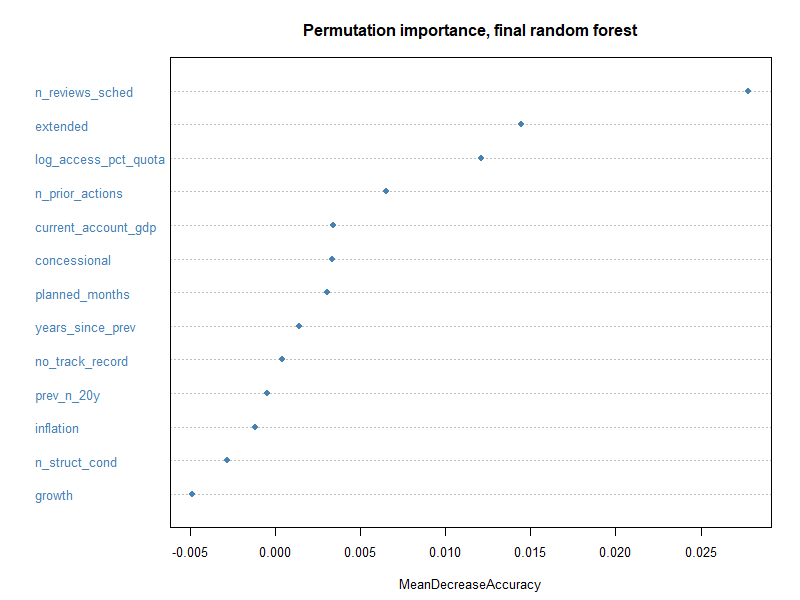
\includegraphics[width=0.82\linewidth]{../Presentation/figures/rf_importance.png}
\refstepcounter{figure}\label{fig:rf-importance}
\wordcaption{\src{Figure \thefigure. Permutation importance of the final forest: mean decrease in out-of-bag accuracy when one input is shuffled (higher values mean more important; values near or below zero mean no contribution)}}
\end{wordtable}

\src{The number of scheduled reviews is the strongest input (Figure~\ref{fig:rf-importance}): 85\% of training programmes with eight or more reviews were interrupted, against 36\% of the others. Part of this is mechanical, as each extra review is one more chance to miss one (Section~\ref{sec:variables}). Because this link is partly built into the outcome, the forest’s training-set signal should be read as an upper bound on what approval-day information reveals about implementation. Programme length receives little importance on its own because it overlaps with the extended indicator (\emph{r} = 0.77); within each facility type, longer training programmes were interrupted more often (all 10 non-extended programmes planned for more than 30 months, against 49\% of those planned for 30 months or less), in line with Reinsberg et al. (2022, p. 1028), who find that longer agreements fail more often. Extended facilities (EFF or ECF) come second, with 38\% of extended training programmes interrupted against 60\% of the others, in line with the IMF’s review: “EFF and EFF-ECF arrangements, generally longer in duration than SBAs, had higher completion rates” (IMF, 2019, p. 45). In our sample the gap mainly reflects ECFs (36\% of training ECFs interrupted), which are also concessional; EFFs alone (57\%) differ little from SBAs (60\%). Section~\ref{sec:policy} discusses whether higher completion in extended programmes reflects better implementation. Access relative to quota ranks third and prior actions fourth (48\% interrupted with at least one prior action, against 37\% without), in line with the IMF’s finding of “a negative association between PAs [prior actions] at arrangement approval and completion rates” (IMF, 2019, p. 45).}

\src{Growth and inflation add no predictive value. Several regression studies find initial economic conditions largely insignificant (Ivanova et al., 2003, p. 1; Reinsberg et al., 2022, p. 1028), although Dreher (2003) reports associations with initial economic vulnerability, and our macro inputs are staff projections, which may be optimistic (Section~\ref{sec:variables}). The literature disagrees on conditionality: Reinsberg et al. (2022, p. 1028) find that structural conditions are associated with interruption, while Ivanova et al. (2003, p. 1) find no material effect. A simple count of structural conditions adds no predictive value in our forest, which therefore cannot test Reinsberg et al.’s finding on specific condition types. These importances describe patterns in the training sample that did not carry over clearly to the test period, and most values outside the top three are close to zero. Section~\ref{sec:alternatives} asks whether a simpler or a more flexible model does better.}

% Verbatim source: Report/initial/Logistic Regression with References.docx
\addsec{\src{Alternative Model: Logistic Regression}}

\src{To evaluate an alternative to the random forest, we used a logistic regression model to predict whether an IMF lending program would be interrupted. We chose logistic regression because the dependent variable, \emph{interrupted}, is binary (Hosmer et al., 2013, p. 1; James et al., 2013, pp. 130–131). It provides a relatively simple and interpretable benchmark against which the performance of a more complex model can be analyzed.}

\src{The model was trained on the same 13 explanatory variables as the random forest, covering program design, conditionality, previous program experience and macroeconomic conditions. These include economic growth, inflation, whether an arrangement is extended or concessional, and the number of prior actions required before approval. The model estimates the probability of an interruption, which is converted into a binary prediction using a threshold of 0.50 (James et al., 2013, p. 146). It was not tuned, while the random forest was tuned and its threshold searched out of fold. The same training and test sets were used for both models, allowing a direct comparison.}

\src{On the test set of 28 programs, logistic regression achieved an accuracy of 0.536, a balanced accuracy of 0.570 and an AUC of 0.684, against 0.500, 0.508 and 0.586 for the random forest at its selected threshold of 0.51. At the same 0.50 threshold, however, the forest reaches 0.571 and 0.567, so the two models differ mainly in AUC, which does not depend on the threshold (Fawcett, 2006): logistic regression ranks interrupted programs above completed ones more consistently. With 28 test programs, even this gap should be read cautiously, and both results show that predicting interruptions remains difficult.}

\src{A key advantage of logistic regression is its interpretability. Its coefficients indicate how each explanatory variable is associated with the log-odds of interruption, holding the other variables constant (Hosmer et al., 2013, pp. 49–52; see Figure 1). The largest coefficients belong to extended facilities (−4.18, \emph{p} = .004) and concessional facilities (2.31, \emph{p} = .087), of which only the former is statistically significant at the 5\% level. These two variables are strongly correlated in the training data (\emph{r} = .81). As a result, the model splits their joint association into opposite signs and estimates both with large standard errors, so their individual coefficients should not be read in isolation (James et al., 2013, pp. 99–102). The absence of a track record also has a sizeable positive coefficient (1.31), but it is imprecisely estimated (\emph{p} = .231). More generally, these associations are not causal, and coefficient magnitudes are not directly comparable because the predictors are measured on different scales (Hosmer et al., 2013, pp. 62–64).}

\begin{wordtable}
\wordcaption{\src{Figure 1}\par
\src{\emph{Logistic Regression Coefficients for Program Interruption}}}
{\centering
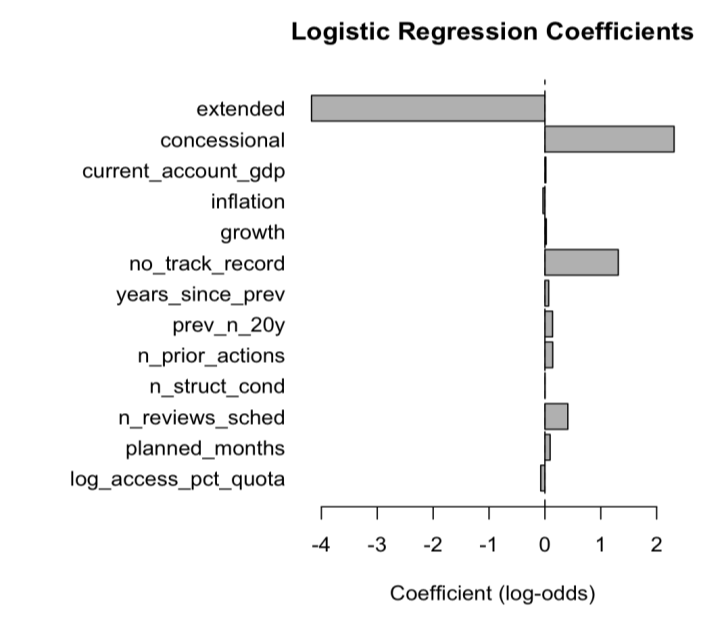
\includegraphics[width=0.78\linewidth]{../Presentation/figures/logit_coefficients.png}\par}
\smallskip
{\footnotesize\src{\emph{Note.} Coefficients are in log-odds and estimated on the training set. Positive values indicate higher odds of interruption. Predictors are on different scales, so bar lengths are not directly comparable measures of importance. Extended and concessional are strongly correlated (\emph{r} = .81).}\par}
\end{wordtable}

\src{The random forest, in contrast, can capture non-linear relationships and interactions between variables (Breiman, 2001a), at the cost of interpretability (Breiman, 2001b; James et al., 2013, pp. 24–26). Logistic regression imposes a simpler functional form and provides a more transparent account of the relationships it represents.}

\src{Overall, logistic regression matched the random forest on balanced accuracy and ranked programs better, while offering greater interpretability. One possible explanation is that the simpler model generalized better, whereas the random forest’s flexibility may have made it more susceptible to fitting noise in the training data (Hastie et al., 2009, pp. 219–223; James et al., 2013, pp. 33–36). However, this cannot be established from the results alone, and with only 28 test programs the differences should be interpreted cautiously. The comparison shows that a more complex model does not necessarily produce better predictions (Christodoulou et al., 2019; Couronné et al., 2018), and that interpretability remains an important consideration when evaluating models for financial decision-making (Rudin, 2019).}

% Verbatim source: Report/initial/3b_Neural_Network_full.docx
\addsec{\src{Model and Set-up}}

\src{A feedforward neural network passes the inputs through layers of neurons, each of which-h applies a non-linear activation function, such as the sigmoid, to a weighted sum of its inputs. This non-linearity is what lets the network learn non-linear relationships (Wüthrich \& Merz, 2023, pp. 269-273). We use the R package nnet, which fits networks with a single hidden layer and optimises the weights with the BFGS method (Ripley \& Venables, 2026). Since flexible networks can also fit the noise in the training data, we keep the network small and add weight decay, which can improve generalisation (Krogh \& Hertz, 1992, p. 950). The 13 predictors are rescaled to [0, 1], as inputs on similar scales help the weights learn at a similar rate (LeCun et al., 1998, Sect. 4.3). The minimum and maximum come from the training set only, so that no information from the test set leaks into the model (Kapoor \& Narayanan, 2023, pp. 1-3).}

\addsubsec{\src{Tuning and Threshold Selection}}

\src{We tune the number of hidden neurons (1, 2, 3 or 5) and the weight decay (0.01, 0.1, 0.5 or 1) with the caret package (Kuhn, 2008). As for the random forest, we use 10-fold cross-validation in which all programmes of a country stay in the same fold, because randomly split folds give over-optimistic error estimates and favour overly complex models when observations are dependent (Roberts et al., 2017, p. 914). Models are compared by balanced accuracy, the mean of sensitivity and specificity, because plain accuracy gives an optimistic estimate for a biased classifier on imbalanced data (Brodersen et al., 2010, p. 3121).}

\begin{wordtable}
\centering
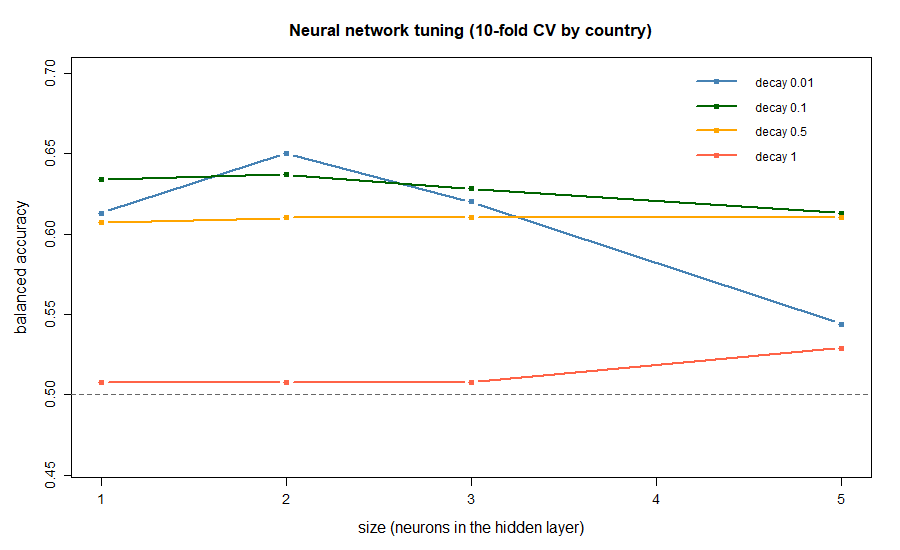
\includegraphics[width=0.94\linewidth]{../Neural_Network/fig_nn_tuning.png}
\wordcaption{\src{\textbf{Figure 1:} Cross-validated balanced accuracy by number of hidden neurons and weight decay (10-fold CV by country, 145 training programmes; dashed line = 0.500).}}
\end{wordtable}

\src{The best network has two hidden neurons and a decay of 0.010, with a cross-validated balanced accuracy of 0.650 (Figure 1). With the same light decay, five neurons only reach 0.544, while a strong decay of 1 keeps every size between 0.510 and 0.530, close to the 0.500 of a model that always predicts the same class. With 145 training programmes, a small and lightly regularised network therefore works best. We then choose the classification threshold that maximises balanced accuracy on the out-of-fold predictions, so that the test set plays no role in model selection. This gives a threshold of 0.440 and an out-of-fold balanced accuracy of 0.684.}

\addsubsec{\src{Test-Set Results and Discussion}}

\src{Table~\ref{tab:model-comparison} compares the final network (13 inputs, 2 hidden neurons, 31 weights) with the group's other models on the 28 test programmes approved between 2014 and 2016. The AUC is the probability that a model ranks a randomly chosen interrupted programme above a randomly chosen completed one, so 0.500 corresponds to random guessing (Fawcett, 2006, p. 867).}

\begin{wordtable}
\wordtablecaption{tab:model-comparison}{\src{\textbf{Table \thetable:} Test-set performance of all models (28 programmes, 2014–2016).}}
\begin{tabularx}{\linewidth}{@{}Xrrrrr@{}}
\toprule
\textbf{\src{Model}} & \textbf{\src{Accuracy}} & \textbf{\src{Sensitivity}} & \textbf{\src{Specificity}} & \textbf{\src{Bal. acc.}} & \textbf{\src{AUC}}\\
\midrule
\src{Neural network} & \src{0.500} & \src{0.294} & \src{0.818} & \src{0.556} & \src{0.567}\\
\src{Random forest (tuned)} & \src{0.500} & \src{0.471} & \src{0.545} & \src{0.508} & \src{0.586}\\
\src{Logistic regression} & \src{0.536} & \src{0.412} & \src{0.727} & \src{0.570} & \src{0.684}\\
\src{Baseline (always interrupted)} & \src{0.607} & \src{1.000} & \src{0.000} & \src{0.500} & \src{0.500}\\
\bottomrule
\end{tabularx}
\end{wordtable}

\src{The network beats the random forest on balanced accuracy (0.556 vs 0.508) but not on AUC (0.567 vs 0.586), and both reach an accuracy of only 0.500, below the 0.607 of predicting an interruption for every programme. The two models also make different errors: the network rarely predicts an interruption (sensitivity 0.294, specificity 0.818), while the forest is more balanced (0.471 and 0.545). The network's result is also fragile. With the default threshold of 0.50 it scores slightly higher on the test set (0.572), and refitting it with 20 different random seeds gives test balanced accuracies between 0.436 and 0.559 (median 0.553). This is expected, since the starting weights are drawn randomly (Wüthrich \& Merz, 2023, p. 284) and the fitted network is not unique.}

\src{We thus find no reliable winner between the two models. With 17 interrupted and 11 completed programmes in the test set, one additional correct prediction moves balanced accuracy by 0.030 to 0.050, as much as the gap between them. The network's balanced accuracy also falls from 0.684 out of fold to 0.556 on the test set, a period in which the share of interrupted programmes rises from 45\% to 61\%. These results are in line with evidence that tree-based models still outperform deep learning on medium-sized tabular datasets of around 10,000 observations (Grinsztajn et al., 2022, p. 507), far more than our 145. Interpretability points the same way: for high-stakes decisions, Rudin (2019) argues for inherently interpretable models over black boxes that are too complicated for humans to comprehend, and the network's 31 weights have no direct economic meaning. Since it brings no clear accuracy gain over the random forest, nor over logistic regression, which has the highest balanced accuracy and AUC in Table~\ref{tab:model-comparison}, we would not use the neural network to flag programmes at risk of interruption.}

\clearpage
% The authors' existing Remarks are merged with Part 6c, rather than replaced.
\section{\src{Discussion and conclusion}}\label{sec:discussion}
\subsection{\src{Summary of findings}}\label{sec:findings}

\src{Using 173 IMF programmes approved in 2002–2016, we asked whether approval-day information can predict whether a conditional lending programme is later interrupted. Our answer is that approval-day information predicts interruption only weakly, and none of the three models is reliably better than the others. On the 28 test programmes, balanced accuracy ranges from 0.51 to 0.57 at thresholds of 0.51 for the forest, 0.50 for logistic regression and 0.44 for the network, against 0.500 for the always-interrupted baseline. At a common threshold of 0.50, the random forest (0.567), the logistic regression (0.570) and the neural network (0.572) lie within 0.005 of each other, while one additional correct prediction moves balanced accuracy by about 0.03 to 0.05. Logistic regression has the highest AUC (0.684).}

\src{Using 13 inputs available at programme approval, we fitted a random forest to predict IMF programme interruptions. Country-grouped cross-validation selected 250 trees and three candidate inputs per split. The final model reached a pooled training out-of-fold balanced accuracy of 0.630, but only 0.508 on the 28 later test programmes at the selected threshold of 0.51. Scheduled reviews, extended facilities and access relative to quota had the highest estimated permutation importance, although these rankings do not establish causal effects. Prior actions rank next.}

\subsection{\src{Limitations}}\label{sec:limitations}

\src{\textbf{Parallel and successive programmes.} Each programme is one observation. Blends approved for the same country on the same day share one review schedule and are merged into one programme. Programmes that overlap or follow an earlier programme of the same country are kept as separate observations: 13 programmes (11 of them in the training set) overlap an earlier one, and 43 of the 84 training countries have more than one programme. Their history enters the models through the track-record inputs. A programme cancelled early and replaced by a successor arrangement counts as interrupted, so the label groups failures with some programmes that were superseded. Because programmes of one country are not independent, we tune the models with country-grouped cross-validation; the test set, by contrast, draws 26 of its 28 programmes from countries in the training set, so it measures prediction for later programmes of mostly known borrowers.}

\src{\textbf{Other limitations.} The results are limited by the small test sample, the change in interruption frequency between training and testing, and the use of training validation results for both model and threshold selection. Test classifications are also sensitive to the threshold: moving from 0.50 to 0.51 changes two predictions. Furthermore, scheduled reviews enter the outcome definition, giving their predictive importance a partly mechanical basis. The macroeconomic inputs are staff projections, and a few extreme values, such as Yemen’s 2014 inflation of −17.7\%, may reflect recording issues in MONA. Our inputs do not measure elections, political cohesion or bureaucratic quality (Dreher, 2003; Ivanova et al., 2003). The share of interrupted programmes rises from 44.8\% in the training set to 60.7\% in the test set, and test programmes are larger, longer and less often concessional, so the drop in performance may reflect a change in the population as well as overfitting.}

\subsection{\src{Policy implications}}\label{sec:policy}

\src{Until performance is shown to be stable across further samples, this forest is best regarded as an exploratory model rather than a dependable stand-alone signal for sovereign-risk decisions. At most, such a score could complement staff judgement. The importance of scheduled reviews must not be read as a reason to schedule fewer reviews: part of the link is mechanical, and fewer reviews would lower measured interruption without improving implementation.}

\src{Extended programmes (EFF or ECF) were interrupted less often than others (38\% against 60\% in the training set), mainly because of ECFs (36\%); EFFs (57\%) differ little from SBAs (60\%). Higher completion in extended programmes need not mean better implementation. Long lending relationships can create moral hazard: a borrower that expects waivers, modified targets or lenient reviews has a weaker incentive to implement, and a lender that has supported a country for years may hesitate to interrupt its programme. The IMF’s Independent Evaluation Office examined such prolonged use of IMF resources (Independent Evaluation Office of the International Monetary Fund [IEO], 2002 [p. ?]), and Reinsberg et al. (2022) use the term “dependency trap” in the title of their study. Because our outcome counts completed reviews, it cannot separate compliance from leniency, so high completion in long programmes is weak evidence of success on its own.}

\subsection{\src{Further research}}\label{sec:further-research}

\src{Future work could expand the sample, assess performance over additional chronological splits, and investigate richer approval-day indicators of political commitment and institutional capacity. A natural next step is to examine a different time period. MONA review records start in 2002, so earlier arrangements would need review histories from other IMF sources, while programmes approved after 2016, including those of the COVID-19 period, can be added once they have run their course. A longer sample would allow rolling time-ordered splits, which train on earlier approval years and test on the following ones and would show whether the weak test result reflects the 2014–2016 period, the small test set or a general lack of signal. Preprocessing and model selection should be confined to the training portions of validation splits.}

\src{Further work could add political and institutional inputs (Dreher, 2003; Ivanova et al., 2003). Coding the type of each condition instead of counting conditions would allow a test of Reinsberg et al. (2022), who associate specific types, such as public-sector reform and privatisation, with interruption. Re-estimating the models without the number of scheduled reviews would show how much of the signal is mechanical, and review-level data would allow predicting each review’s completion with the information available at that review.}

\clearpage
% Consolidated from the six reference lists in the current Word documents.
% Each retained entry preserves a source version verbatim. Duplicate works
% appear once, using the source entry with the fuller publication/link details.
% The IMF 2026a/b/c labels follow the reviewed study-design document.
% Breiman's 2001a/b labels follow the updated logistic-regression document.
\addsec{References}\label{sec:references}
\begin{wordreferences}
\src{Abedin, M. Z., Hassan, M. K., Hájek, P., \& Uddin, M. M. (2021). \emph{The Essentials of Machine Learning in Finance and Accounting. Routledge}. \url{https://doi.org/10.4324/9781003037903}}

\src{Agbloyor, E. K., Pan, L., Dwumfour, R. A., \& Gyeke-Dako, A. (2023). We are back again! What can artificial intelligence and machine learning models tell us about why countries knock at the door of the IMF? Finance Research Letters, 57, 104244. \url{https://doi.org/10.1016/j.frl.2023.104244}}

\src{Batsuuri, T., He, S., Hu, R., Leslie, J., \& Lutz, F. (2024). Predicting IMF-supported programs: A machine learning approach (IMF Working Paper No. 2024/054). International Monetary Fund. \url{https://www.imf.org/en/Publications/WP/Issues/2024/03/09/Predicting-IMF-Supported-Programs-A-Machine-Learning-Approach-545753}}

\src{Breiman, L. (2001a). Random forests. \emph{Machine Learning, 45}(1), 5–32. \url{https://doi.org/10.1023/A:1010933404324}}

\src{Breiman, L. (2001b). Statistical modeling: The two cultures. \emph{Statistical Science, 16}(3), 199–231. \url{https://doi.org/10.1214/ss/1009213726}}

\src{Brodersen, K. H., Ong, C. S., Stephan, K. E., \& Buhmann, J. M. (2010). The balanced accuracy and its posterior distribution. In Proceedings of the 20th International Conference on Pattern Recognition (pp. 3121–3124). IEEE. \url{https://doi.org/10.1109/ICPR.2010.764}}

\src{Christodoulou, E., Ma, J., Collins, G. S., Steyerberg, E. W., Verbakel, J. Y., \& Van Calster, B. (2019). A systematic review shows no performance benefit of machine learning over logistic regression for clinical prediction models. \emph{Journal of Clinical Epidemiology, 110}, 12–22. \url{https://doi.org/10.1016/j.jclinepi.2019.02.004}}

\src{Couronné, R., Probst, P., \& Boulesteix, A.-L. (2018). Random forest versus logistic regression: A large-scale benchmark experiment. \emph{BMC Bioinformatics, 19}, Article 270. \url{https://doi.org/10.1186/s12859-018-2264-5}}

\src{Dreher, A. (2003). The influence of elections on IMF programme interruptions. The Journal of Development Studies, 39(6), 101–120. \url{https://doi.org/10.1080/00220380312331293597}}

\src{Dreher, A. (2009). IMF conditionality: Theory and evidence. Public Choice, 141, 233–267. \url{https://doi.org/10.1007/s11127-009-9486-z}}

\src{Fawcett, T. (2006). An introduction to ROC analysis. Pattern Recognition Letters, 27(8), 861–874. \url{https://doi.org/10.1016/j.patrec.2005.10.010}}

\src{Grinsztajn, L., Oyallon, E., \& Varoquaux, G. (2022). Why do tree-based models still outperform deep learning on typical tabular data? Advances in Neural Information Processing Systems, 35, 507–520.}

\src{Gu, S., Kelly, B., \& Xiu, D. (2020). Empirical asset pricing via machine learning. The Review of Financial Studies, 33(5), 2223–2273. \url{https://doi.org/10.1093/rfs/hhaa009}}

\src{Hastie, T., Tibshirani, R., \& Friedman, J. (2009). \emph{The elements of statistical learning: Data mining, inference, and prediction} (2nd ed.). Springer. \url{https://doi.org/10.1007/978-0-387-84858-7}}

\src{He, H., \& Garcia, E. A. (2009). Learning from imbalanced data. IEEE Transactions on Knowledge and Data Engineering, 21(9), 1263–1284. \url{https://doi.org/10.1109/TKDE.2008.239}}

\src{Hosmer, D. W., Lemeshow, S., \& Sturdivant, R. X. (2013). \emph{Applied logistic regression} (3rd ed.). Wiley. \url{https://doi.org/10.1002/9781118548387}}

\src{Independent Evaluation Office of the International Monetary Fund. (2002). \emph{Evaluation of prolonged use of IMF resources}. International Monetary Fund.}

\src{International Monetary Fund. (2019). \emph{2018 review of program design and conditionality} (IMF Policy Paper No. 19/012). International Monetary Fund. \url{https://www.imf.org/-/media/Files/Publications/PP/2019/PPEA2019012.ashx}}

\src{International Monetary Fund. (2026a). IMF financial data query tool: History of lending arrangements [Data set]. Retrieved September 18, 2026, from \url{https://www.imf.org/external/np/fin/tad/query.aspx}}

\src{International Monetary Fund. (2026b). Monitoring of Fund Arrangements (MONA) database [Data set]. Retrieved September 18, 2026, from \url{https://www.imf.org/external/np/pdr/mona/index.aspx}}

\src{International Monetary Fund. (2026c). World Economic Outlook database: April 2026 edition [Data set]. Retrieved [date ?], from \url{https://www.imf.org/en/Publications/WEO/weo-database/2026/April}}

\src{International Monetary Fund. (n.d.). IMF conditionality [Fact sheet]. Retrieved October 13, 2026, from \url{https://www.imf.org/en/About/Factsheets/Sheets/2023/IMF-Conditionality}}

\src{Iseringhausen, M., Nkusu, M., \& Wiranto, W. (2019). Repeated use of IMF-supported programs: Determinants and forecasting (IMF Working Paper No. 2019/245). International Monetary Fund. \url{https://doi.org/10.5089/9781513511689.001}}

\src{Ivanova, A., Mayer, W., Mourmouras, A., \& Anayiotos, G. (2003). What determines the implementation of IMF-supported programs? (IMF Working Paper No. 2003/008). International Monetary Fund. \url{https://doi.org/10.5089/9781451842531.001}}

\src{James, G., Witten, D., Hastie, T., \& Tibshirani, R. (2013). An introduction to statistical learning: With applications in R. Springer. \url{https://doi.org/10.1007/978-1-4614-7138-7}}

\src{Joyce, J. P. (2006). Promises made, promises broken: A model of IMF program implementation. Economics \& Politics, 18(3), 339–365. \url{https://doi.org/10.1111/j.1468-0343.2006.00173.x}}

\src{Kapoor, S., \& Narayanan, A. (2023). Leakage and the reproducibility crisis in machine-learning-based science. Patterns, 4(9), 100804. \url{https://doi.org/10.1016/j.patter.2023.100804}}

\src{Krogh, A., \& Hertz, J. A. (1992). A simple weight decay can improve generalization. Advances in Neural Information Processing Systems, 4, 950–957.}

\src{Kuhn, M. (2008). Building predictive models in R using the caret package. Journal of Statistical Software, 28(5), 1–26. \url{https://doi.org/10.18637/jss.v028.i05}}

\src{LeCun, Y., Bottou, L., Orr, G. B., \& Müller, K.-R. (1998). Efficient BackProp. In G. B. Orr \& K.-R. Müller (Eds.), Neural networks: Tricks of the trade (pp. 9–50). Springer. \url{https://doi.org/10.1007/3-540-49430-8_2}}

\src{Liaw, A., \& Wiener, M. (2002). Classification and regression by randomForest. \emph{R News, 2}(3), 18–22.}

\src{Mody, A., \& Saravia, D. (2006). Catalysing private capital flows: Do IMF programmes work as commitment devices? The Economic Journal, 116(513), 843–867. \url{https://doi.org/10.1111/j.1468-0297.2006.01114.x}}

\src{Reinsberg, B., Stubbs, T., \& Kentikelenis, A. (2022). Compliance, defiance, and the dependency trap: International Monetary Fund program interruptions and their impact on capital markets. Regulation \& Governance, 16(4), 1022–1041. \url{https://doi.org/10.1111/rego.12422}}

\src{Ripley, B. D., \& Venables, W. N. (2026). nnet: Feed-forward neural networks and multinomial log-linear models (R package version 7.3-21) [Computer software]. \url{https://CRAN.R-project.org/package=nnet}}

\src{Roberts, D. R., Bahn, V., Ciuti, S., Boyce, M. S., Elith, J., Guillera-Arroita, G., Hauenstein, S., Lahoz-Monfort, J. J., Schröder, B., Thuiller, W., Warton, D. I., Wintle, B. A., Hartig, F., \& Dormann, C. F. (2017). Cross-validation strategies for data with temporal, spatial, hierarchical, or phylogenetic structure. Ecography, 40(8), 913–929. \url{https://doi.org/10.1111/ecog.02881}}

\src{Rudin, C. (2019). Stop explaining black box machine learning models for high stakes decisions and use interpretable models instead. Nature Machine Intelligence, 1(5), 206–215. \url{https://doi.org/10.1038/s42256-019-0048-x}}

\src{Shmueli, G. (2010). To explain or to predict? Statistical Science, 25(3), 289–310. \url{https://doi.org/10.1214/10-STS330}}

\src{Venables, W. N., \& Ripley, B. D. (2002). \emph{Modern applied statistics with S} (4th ed.). Springer.}

\src{World Bank. (2026). World Development Indicators [Data set]. Retrieved September 18, 2026, from \url{https://databank.worldbank.org/source/world-development-indicators}}

\src{Wüthrich, M. V., \& Merz, M. (2023). Statistical foundations of actuarial learning and its applications. Springer. \url{https://doi.org/10.1007/978-3-031-12409-9}}
\end{wordreferences}

\clearpage
% Based on the List of Aids in
% Report/initial/Declaration_of_Authorship_We_With_Aids_and_Signatures.docx;
% AI-use descriptions updated and EndNote use confirmed by the authors.
\addsec{\src{Declaration of AI use}}\label{sec:ai-use}
\addsubsec{\src{List of Aids}}

\begin{wordtable}
\renewcommand{\arraystretch}{1.4}
\begin{tabularx}{\linewidth}{@{}L{0.20\linewidth}>{\raggedright\arraybackslash}XL{0.24\linewidth}@{}}
\toprule
\textbf{\src{Resource}} & \textbf{\src{Use}} & \textbf{\src{Affected Section}}\\
\midrule
\src{EndNote} & \src{Reference and citation management} & \src{Entire report}\\
\addlinespace[9pt]
\src{ChatGPT (OpenAI)} & \src{Help with correcting and designing code, including R code debugging; literature search; review and editing of drafts, including grammar, spelling and rephrasing.} & \src{Entire report + code}\\
\addlinespace[9pt]
\src{Claude (Anthropic)} & \src{Help with correcting and designing code, including R code debugging; literature search; review and editing of drafts, including grammar, spelling and rephrasing.} & \src{Entire report + code}\\
\bottomrule
\end{tabularx}
\end{wordtable}

\clearpage
% Verbatim declaration from
% Report/initial/Declaration_of_Authorship_We_With_Aids_and_Signatures.docx
\addsec{\src{Declaration of Authorship}}

\src{The following text is to be attached to the thesis.}

\src{“We hereby declare,}

\begin{itemize}[leftmargin=1.5em,label=\textbullet,itemsep=6pt,parsep=0pt,topsep=8pt,partopsep=0pt]
\item \src{that we have written this thesis independently,}

\item \src{that we have written the thesis using only the aids specified in the index;}

\item \src{that all parts of the thesis produced with the help of aids have been declared;}

\item \src{that we have handled both input and output responsibly when using AI. We confirm that we have therefore only read in public data or data released with consent and that we have checked, declared and comprehensibly referenced all results and/or other forms of AI assistance in the required form and that we are aware that we are responsible if incorrect content, violations of data protection law, copyright law or scientific misconduct (e.g. plagiarism) have also occurred unintentionally;}

\item \src{that we have mentioned all sources used and cited them correctly according to established academic citation rules;}

\item \src{that we have acquired all immaterial rights to any materials we may have used, such as images or graphics, or that these materials were created by us;}

\item \src{that the topic, the thesis or parts of it have not already been the object of any work or examination of another course, unless this has been expressly agreed with the faculty member in advance and is stated as such in the thesis;}

\item \src{that we are aware of the legal provisions regarding the publication and dissemination of parts or the entire thesis and that we comply with them accordingly;}

\item \src{that we are aware that our thesis can be electronically checked for plagiarism and for third-party authorship of human or technical origin and that we hereby grant the University of St.Gallen the copyright according to the Examination Regulations as far as it is necessary for the administrative actions;}

\item \src{that we are aware that the University will prosecute a violation of this Declaration of Authorship and that disciplinary as well as criminal consequences may result, which may lead to expulsion from the University or to the withdrawal of our titles.”}
\end{itemize}

\src{By submitting this thesis, we confirm through our conclusive actions that we are submitting the Declaration of Authorship, that we have read and understood it, and that it is true.}

\end{document}
